%
% 1-fundamtenallemma.tex
%
% (c) 2023 Prof Dr Andreas Müller
%

%
% Integration
%
\subsection{Partielle Integration}
Die partielle Integration für ein Integral einer Variablen
transformiert das Integral
\[
\int_{a}^{b} f(x) g'(x)\,dx
\]
in die Summe
\[
\biggl[ f(x) g(x) \biggr]_a^b
-
\int_a^b f'(x) g(x)\,dx.
\]
Der erste Term hängt nur von Informationen auf dem Rand des 
Definitionsbereichs ab.
Eine Verallgemeinerung dieser Regel muss vor allem auch klären,
wie dieser erste Term aussehen soll.
Er darf nur von den Funktionswerten der Funktionen auf dem Rand
$\partial\Omega$ abhängen.
Die Abhängigkeit muss ausserdem linear sein.
In diesem Abschnitt sollen in einer Folge von Beispielen die
wichtigsten Fälle systematisch entwickelt werden.

%
% Ableitung von Produkten
%
\subsubsection{Ableitung von Produkten}
Die Regel für die partielle Integration von Produkten von Funktionen
einer Variable ist die Integralform der Produktregel
\[
\frac{d}{dx}(f(x)g(x)) = f'(x)g(x) + f(x)g'(x).
\]
Für eine Erweiterung auf ist daher als erstes zu klären, welche Art
von Differentialoperatoren überhaupt in Frage kommen.

Die partielle Ableitung nach einer der Variablen bei Funktionen
$f$ und $g$ von $n$ Variablen erfüllt eine Produktregel:
\[
\frac{\partial}{\partial x_k}
(f(x)g(x))
=
\frac{\partial f}{\partial x_k}(x)\,g(x)
+
f(x)
\,
\frac{\partial g}{\partial x_k}(x)
\]
für jedes $k=1,\dots,n$.
Die partiellen Ableitungen sind aber nur von untergeordnetem Interesse,
da sie für sich allein von der Wahl des Koordinatensystems abhängig 
sind und daher zum Beispiel keine koordinatenunabhängige physikalische
Bedeutung haben können.

Der Gradient wurde aus der Richtungsableitung konstruiert und es wurde
gezeigt, dass 
\[
\operatorname{grad} f(x)
=
\begin{pmatrix}
\frac{\partial f}{\partial x_1}\\
\vdots\\
\frac{\partial f}{\partial x_n}
\end{pmatrix}
\]
eine koordinatenunabhängige Bedeutung als der Vektor hat, in dessen
Richtung die schnellste Zunahme der Funktion $f$ erfolgt.
Und tatsächlich gilt auch für den Gradienten eine Produktformel:
\begin{align*}
\operatorname{grad}(f(x)g(x))
&=
\begin{pmatrix}
\frac{\partial}{\partial x_1}(f(x)g(x))\\
\vdots\\
\frac{\partial}{\partial x_n}(f(x)g(x))
\end{pmatrix}
=
\begin{pmatrix}
\frac{\partial f}{\partial x_1} g(x)
+
f(x) \frac{\partial g}{\partial x_1}\\
\vdots\\
\frac{\partial f}{\partial x_n} g(x)
+
f(x) \frac{\partial g}{\partial x_n}
\end{pmatrix}
\\
&=
(\operatorname{grad}f(x)) g(x)
+
f(x)(\operatorname{grad}g(x))
\end{align*}
Wir haben also den folgenden Satz hergeleitet.

\begin{satz}[Produktformel für Gradient]
Sind $f$ und $g$ Funktionen $\mathbb{R}^n \to\mathbb{R}$, dann gilt
\[
\grad (fg) = (\grad f)g + f\grad g.
\]
\end{satz}

%
% Divergenz
%
\subsubsection{Divergenz}
Der Gradient einer Funktion $f\colon\mathbb{R}^n\to\mathbb{R}$ ist
ein sogenanntes Vektorfeld im Sinne der folgenden Definition.

\begin{definition}[Vektorfeld]
\label{buch:felder:fundamentallemma:def:vektorfeld}
Eine Abbildung $g\colon\mathbb{R}^n\to\mathbb{R}^k$, die jedem Punkt
von $\mathbb{R}^n$ einen $k$-dimensionalen Vektor zuordnet, heisst
ein {\em $k$-dimensionales Vektorfeld}.
\index{Vektorfeld}
\end{definition}

Auch für ein Vektorfeld lassen sich interessante Differentialoperatoren
definieren, deren Bedeutung später klar werden wird.

\begin{definition}[Divergenz]
\label{buch:felder:fundamentallemme:def:divergenz}
Die {\em Divergenz} eines $n$-dimensionalen differenzierbaren
Vektorfeldes $g\colon:\mathbb{R}^n\to\mathbb{R}^n$ ist die Funktion
\[
\operatorname{div} g
\colon
\mathbb{R}^n\to\mathbb{R}
:
x \mapsto
\frac{\partial g_1}{\partial x_1}(x)
+\ldots+
\frac{\partial g_n}{\partial x_n}(x)
=
\sum_{i=1}^n
\frac{\partial g_i}{\partial x_i}(x).
\]
\end{definition}

Auch für die Divergenz gibt es eine Produktformel.
Seien
\[
f\colon\mathbb{R}^3\to\mathbb{R}
\qquad\text{und}\qquad
g\colon\mathbb{R}^3\to\mathbb{R}^3
\]
stetig differenzierbare Funktionen.
Die Komponenten von $g$ schreiben wir $g_i$, $i=1,\dots,n$.

\begin{satz}[Produktformel für Divergenz]
Für 
\[
\operatorname{div}(fg)
=
\grad f \cdot g
+
f\operatorname{div}g.
\]
\end{satz}

\begin{proof}
Wir berechnen die Divergenz von $f\cdot g$:
\begin{align*}
\operatorname{div} fg(x)
&=
\frac{\partial}{\partial x_1}(f(x)g_1(x))
+
\ldots
+
\frac{\partial}{\partial x_n}(f(x)g_n(x))
\\
&=
\frac{\partial f}{\partial x_1}(x)g_1(x)
+f(x)\frac{\partial g_1}{\partial x_1}(x)
+
\ldots
+
\frac{\partial f}{\partial x_n}(x)g_n(x)
+f(x)\frac{\partial g_n}{\partial x_n}(x)
\\
&=
\sum_{i=1}^n \frac{\partial f}{\partial x_i}(x) g_i(x)
+
f(x)
\sum_{i=1}^n \frac{\partial g_i}{\partial x_i}(x)
\\
&=
\grad f(x)\cdot \operatorname{div} g(x)
+
f(x)\operatorname{div}g(x).
\qedhere
\end{align*}
\end{proof}

Die Produktregel sagt also auch hier, dass der Differentialoperator
auf jeden Faktor einzeln angewendet werden kann. 
Je nach Art des Faktors passt aber der Gradient oder die Divergenz.

%
% Laplace-Operator
%
\subsubsection{Laplace-Operator}
Besonderes Interesse an der Divergenz entsteht aus dem Zusammenhang
mit dem Laplace-Operator.

\begin{definition}[Laplace-Operator]
Für eine zweimal stetig differenzierbare Funktion
$f\colon\mathbb{R}^n\to\mathbb{R}$
ist der {\em Laplace-Operator} definiert durch
\[
\Delta f(x)
=
\frac{\partial^2 f}{\partial x_1^2}(x)
+\ldots+
\frac{\partial^2 f}{\partial x_n^2}(x)
=
\sum_{i=1}^n \frac{\partial^2 f}{\partial x_i^2}(x).
\]
\end{definition}

Der Laplace-Operator ist ein Differentialoperator zweiter Ordnung.
Wir berechnen die Zusammensetzung der beiden Differentialoperatorn
erster Ordnung $\operatorname{div}$ und $\grad$
für eine zweimal stetig differenzierbare Funktion
$f\colon\mathbb{R}^n\to\mathbb{R}$ und erhalten
\begin{align*}
\operatorname{div}\grad f(x)
&=
\sum_{i=1}^n
\frac{\partial}{\partial x_i}
\frac{\partial f}{\partial x_i}(x)
=
\frac{\partial^2 f}{\partial x_i^2}(x)
=
\Delta f(x).
\end{align*}
Daraus lässt sich jetzt auch eine Produktformel für den Laplace-Operator
ableiten.
Dazu wenden wir ihn auf das Produkt zweier skalarer Funktionen
$f,g\colon\mathbb{R}^n\to\mathbb{R}$ an:
\begin{align}
\operatorname{div}\grad (fg)(x)
&=
\operatorname{div}\bigl((\grad f(x)) g(x) + f(x)\grad g(x)\bigr)
\intertext{nach der Produktformel für den Gradienten.
Auf die einzelnen Summanden wenden wir jetzt die Produktformel für
die Divergenz an und erhalten}
&=
(\operatorname{div}\grad f(x))g(x) + \grad f(x)\cdot \grad g(x)
\notag
\\
&\qquad\qquad
+
\grad f(x)\cdot\grad g(x) + f(x) \operatorname{div}\grad g(x).
\notag
\intertext{Durch Anwendung der Definition des Laplace-Operators
erhalten wir die gesuchte Produktformel}
\Delta (fg)(x)
&=
(\Delta f(x)) g(x) + 2\grad f(x)\cdot \grad g(x) + f(x)\Delta g(x).
\label{buch:felder:fundamentallemma:eqn:laplaceproduktformel}
\end{align}
Da der Laplace-Operator ein Operator zweiter Ordnung ist, ähnelt 
die rechte Seite von
\eqref{buch:felder:fundamentallemma:eqn:laplaceproduktformel}
der binomischen Formel.

%
% Rotation
%
\subsubsection{Rotation}
In drei Dimensionen gibt es einen weiteren interessanten Differentialoperator,
dessen Konstruktion auf dem Vektorprodukt beruht.

\begin{definition}[Rotation]
Sei $g\colon\mathbb{R}^3\to\mathbb{R}^3$ ein differenzierbares
dreidimensionales Vektorfeld, dann heisst das Vektor
\[
\operatorname{rot}g(x)
=
\begin{pmatrix}
\displaystyle
\frac{\partial g_3}{\partial x_2}
-
\frac{\partial g_2}{\partial x_3}
\\
\displaystyle
\frac{\partial g_1}{\partial x_3}
-
\frac{\partial g_3}{\partial x_1}
\\
\displaystyle
\frac{\partial g_2}{\partial x_1}
-
\frac{\partial g_1}{\partial x_2}
\end{pmatrix}
\]
die {\em Rotation} von $g(x)$.
\end{definition}

Die Rotation $\operatorname{rot}g$ wird im englischen Sprachraum manchmal
auch $\operatorname{curl}g$ geschrieben.
Auch für die Rotation gibt es Produktformeln für die Ableitung.

\begin{satz}[Produktformeln für Rotation]
Sei $f\colon\mathbb{R}^3\to\mathbb{R}$ differenzierbar und
$g,h\colon\mathbb{R}^3\to\mathbb{R}^3$ differenzierbare dreidimensionale
Vektorfelder.
Dann gilt
\begin{align*}
\operatorname{rot}(fg)(x)
&=
\\
\operatorname{rot}(g\times h)(x)
&=
\grad f\times g(x) + f(x)\operatorname{rot}(x).
\end{align*}
\end{satz}

\begin{proof}
Der Beweis erfolgt durch Nachrechnen:
\bgroup
\renewcommand{\arraystretch}{1.9}
\begin{align*}
\operatorname{rot}(fg)(x)
&=
\begin{pmatrix}
\displaystyle
\frac{\partial}{\partial x_2}(fg_3)(x)-\frac{\partial}{\partial x_3}(fg_2)(x)
\\
\displaystyle
\frac{\partial}{\partial x_3}(fg_1)(x)-\frac{\partial}{\partial x_1}(fg_3)(x)
\\
\displaystyle
\frac{\partial}{\partial x_1}(fg_2)(x)-\frac{\partial}{\partial x_2}(fg_1)(x)
\end{pmatrix}
\\
&=
\begin{pmatrix}
\displaystyle
\frac{\partial f}{\partial x_2}(x)g_3(x)
-\frac{\partial f}{\partial x_3}(x)g_2(x)
+
f(x)\biggl(\frac{\partial g_3}{\partial x_2}(x)
-\frac{\partial g_2}{\partial x_3}(x)\biggr)
\\
\displaystyle
\frac{\partial f}{\partial x_3}(x)g_1(x)
-\frac{\partial f}{\partial x_1}(x)g_3(x)
+
f(x)\biggl(\frac{\partial g_1}{\partial x_3}(x)
-\frac{\partial g_3}{\partial x_1}(x)\biggr)
\\
\displaystyle
\frac{\partial f}{\partial x_1}(x)g_2(x)
-\frac{\partial f}{\partial x_2}(x)g_1(x)
+
f(x)\biggl(\frac{\partial g_2}{\partial x_1}(x)
-\frac{\partial g_1}{\partial x_2}(x)\biggr)
\end{pmatrix}
\\[5pt]
&=
(\grad f(x))\times g(x) + f(x)\operatorname{rot}(x).
\qedhere
\end{align*}
\egroup
\end{proof}

%\begin{satz}[Divergenz eines Vektorproduktes]
%\begin{align*}
%\operatorname{div}(g\times h)(x)
%&=
%\end{align*}
%\end{satz}
%
%\begin{proof}
%Durch Nachrechnen
%\begin{align*}
%\operatorname{div}(g\times h)(x)
%&=
%\frac{\partial}{\partial x_1}\bigl(
%g_2(x)h_3(x)-g_3(x)h_2(x)
%\bigr)
%+
%\frac{\partial}{\partial x_2}\bigl(
%g_3(x)h_1(x)-g_1(x)h_3(x)
%\bigr)
%\\
%&\qquad\qquad
%+
%\frac{\partial}{\partial x_3}\bigl(
%g_1(x)h_2(x)-g_2(x)h_1(x)
%\bigr)
%\\
%&=
%\frac{\partial g_2}{\partial x_1}(x)h_3(x)
%-
%g_2(x) \frac{\partial h_3}{\partial x_1}
%+
%\frac{\partial g_3}{\partial x_2}(x)h_1(x)
%-
%g_3(x) \frac{\partial h_1}{\partial x_2}
%\\
%&\qquad\qquad
%+
%\frac{\partial g_1}{\partial x_3}(x)h_2(x)
%-
%g_1(x) \frac{\partial h_2}{\partial x_3}
%\\
%&=
%\frac{\partial g_3}{\partial x_2}(x)h_1(x)
%+
%\frac{\partial g_1}{\partial x_3}(x)h_2(x)
%+
%\frac{\partial g_2}{\partial x_1}(x)h_3(x)
%\\
%&\qquad\qquad
%-
%g_1(x) \frac{\partial h_2}{\partial x_3}
%-
%g_2(x) \frac{\partial h_3}{\partial x_1}
%-
%g_3(x) \frac{\partial h_1}{\partial x_2}
%\\
%&=
%\end{align*}
%\end{proof}

%
% Schreibweise mit dem Nabla-Operator
%
\subsubsection{Schreibweise mit dem Nabla-Operator}
Der Nabla-Operator ist in
Definition~\ref{buch:fuvar:richtungsableitung:def:nabla} als der 
Vektor der partiellen Differentialoperatoren nach den unabhängigen
Variablen eingeführt worden.
Der Gradient einer Funktion $f$ ergab sich dann ganz natürlich als
ein ``Produkt'' des Nabla-Operators mit der Funktion.
Auch die Divergenz und die Rotation lassen sich auf diese Art
schreiben.

\begin{definition}
Ist $g\colon\mathbb{R}^n\to\mathbb{R}^n$ ein differenzierbares
$n$-dimensionales Vektorfeld, dann gilt
\begin{align*}
\operatorname{div}g &= \nabla\cdot g.
\intertext{Für $n=3$ gilt ausserdem}
\operatorname{rot}g &= \nabla\times g.
\end{align*}
\end{definition}

Formal wird die Zusammensetzung von Divergenz und Gradient einer Funktion
$f\colon\mathbb{R}^n\to\mathbb{R}$ 
zu
\[
\operatorname{div}\grad f
=
\nabla\cdot\nabla f
=
\biggl(
\sum_{i=1}^n
\frac{\partial}{\partial x_i}
\frac{\partial}{\partial x_i}
\biggr)
f
=
\sum_{i=1}^n \frac{\partial^2 f}{\partial x_i^2}(x)
=
\Delta f(x)
\]
oder abgekürzt $\nabla\cdot\nabla=\Delta$.
Bekannte Identitäten für Skalar- und Vektorprodukt werden so zu Identitäten
für Differentialoperatoren.
Zum Beispiel ist
\[
\operatorname{rot}\operatorname{grad} f
=
\nabla\times\nabla f
=
0,
\]
da ein Vektorprodukt von zwei gleichen Faktoren verschwindet.

Für das doppelte Kreuzprodukt bekommt man
\begin{align*}
\operatorname{div}\operatorname{rot}g
&=
\nabla\times(\nabla \times g)
=
\nabla\times
{\renewcommand{\arraystretch}{1.9}
\begin{pmatrix}
\displaystyle
\frac{\partial g_3}{\partial x_2}-\frac{\partial g_2}{\partial x_3}\\
\displaystyle
\frac{\partial g_1}{\partial x_3}-\frac{\partial g_3}{\partial x_1}\\
\displaystyle
\frac{\partial g_2}{\partial x_1}-\frac{\partial g_1}{\partial x_2}
\end{pmatrix}}
\\
&=
{\renewcommand{\arraystretch}{1.9}
\begin{pmatrix}
\displaystyle
\frac{\partial}{\partial x_2}
\biggl(
{\color{darkred}\frac{\partial g_2}{\partial x_1}}-
{\color{darkgreen}\frac{\partial g_1}{\partial x_2}}
\biggr)
-
\frac{\partial}{\partial x_3}
\biggl(
{\color{orange}\frac{\partial g_1}{\partial x_3}}-
{\color{blue}\frac{\partial g_3}{\partial x_1}}
\biggr)
\\
\displaystyle
\frac{\partial}{\partial x_3}
\biggl(
{\color{darkred}\frac{\partial g_3}{\partial x_2}}-
{\color{darkgreen}\frac{\partial g_2}{\partial x_3}}
\biggr)
-
\frac{\partial}{\partial x_1}
\biggl(
{\color{orange}\frac{\partial g_2}{\partial x_1}}-
{\color{blue}\frac{\partial g_1}{\partial x_2}}
\biggr)
\\
\displaystyle
\frac{\partial}{\partial x_1}
\biggl(
{\color{darkred}\frac{\partial g_1}{\partial x_3}}-
{\color{darkgreen}\frac{\partial g_3}{\partial x_1}}
\biggr)
-
\frac{\partial}{\partial x_2}
\biggl(
{\color{orange}\frac{\partial g_3}{\partial x_2}}-
{\color{blue}\frac{\partial g_2}{\partial x_3}}
\biggr)
\end{pmatrix}}
\\
&=
{\renewcommand{\arraystretch}{1.9}
\begin{pmatrix}
\displaystyle
{\color{gray}\frac{\partial g_1}{\partial x_1^2}}
+
{\color{darkred}\frac{\partial g_2}{\partial x_1\,\partial x_2}}
+{\color{blue}\frac{\partial g_3}{\partial x_1\,\partial x_3}}
{\color{gray}\mathstrut-\frac{\partial g_1}{\partial x_1^2}}
-{\color{darkgreen}\frac{\partial g_1}{\partial x_2^2}}
-{\color{orange}\frac{\partial g_1}{\partial x_3^2}}
\\
\displaystyle
{\color{blue}\frac{\partial g_1}{\partial x_1\,\partial x_2}}
{\color{gray}\mathstrut+\frac{\partial g_2}{\partial x_2^2}}
+{\color{darkred}\frac{\partial g_3}{\partial x_2\,\partial x_3}}
-{\color{orange}\frac{\partial g_2}{\partial x_1^2}}
{\color{gray}\mathstrut-\frac{\partial g_2}{\partial x_2^2}}
-{\color{darkgreen}\frac{\partial g_2}{\partial x_3^2}}
\\
\displaystyle
{\color{darkred}\frac{\partial g_1}{\partial x_1\,\partial x_3}}
+{\color{blue}\frac{\partial g_2}{\partial x_2\,\partial x_3}}
{\color{gray}\mathstrut+\frac{\partial g_3}{\partial x_3^2}}
-{\color{darkgreen}\frac{\partial g_3}{\partial x_1^2}}
-{\color{orange}\frac{\partial g_3}{\partial x_2^2}}
{\color{gray}\mathstrut-\frac{\partial g_3}{\partial x_2^2}}
\end{pmatrix}}.
\intertext{Die Farben der Terme deuten an, aus welchem Term im 
vorangegangenen Ausdruck sie hervorgegangen sind.
Die grauen Terme wurden ergänzt und heben sich jeweils weg, sie
ändern also den Ausdruck nicht, helfen aber, die Komponenten
mit Hilfe von bekannten Differentialoperatoren zu schreiben:
}
&=
{\renewcommand{\arraystretch}{1.9}
\begin{pmatrix}
\displaystyle
\frac{\partial}{\partial x_1}\biggl(
{\color{gray}\frac{\partial g_1}{\partial x_1}}
+
{\color{darkred}\frac{\partial g_2}{\partial x_2}}
+
{\color{blue}\frac{\partial g_3}{\partial x_3}}
\biggr)
-\Delta g_1
\\
\displaystyle
\frac{\partial}{\partial x_2}\biggl(
{\color{blue}\frac{\partial g_1}{\partial x_1}}
+
{\color{gray}\frac{\partial g_2}{\partial x_2}}
+
{\color{darkred}\frac{\partial g_3}{\partial x_3}}
\biggr)
-\Delta g_2
\\
\displaystyle
\frac{\partial}{\partial x_3}\biggl(
\smash{\underbrace{
{\color{darkred}\frac{\partial g_1}{\partial x_1}}
+
{\color{blue}\frac{\partial g_2}{\partial x_2}}
+
{\color{gray}\frac{\partial g_3}{\partial x_3}}
}_{\displaystyle=\operatorname{div}g}}
\biggr)
-\Delta g_3
\end{pmatrix}}
\\[20pt]
&=
\grad\operatorname{div} g - \Delta g
=
\nabla(\nabla\cdot g) - (\nabla\cdot\nabla) g,
\end{align*}
dies entspricht der Grassmann-Identität
\index{Grassmann-Identität}%
\[
\vec{a}\times(\vec{b}\times\vec{c})
=
\vec{b}(\vec{a}\cdot\vec{c}) - (\vec{a}\cdot\vec{v})\vec{c}
\]
für das doppelte Vektorprodukt mit $\vec{a}=\nabla$, $\vec{b}=\nabla$
und $\vec{c}=g$.


%
% Der Satz von Green
%
\subsubsection{Der Satz von Green}
Der Hauptsatz der Integralrechnung besagt, dass das Integral
einer Ableitung $f'(x)$ über ein Intervall $[a,b]$ durch die
Funktionswerte auf den Endpunkten des Intervalls gegeben ist,
in Formeln
\[
\int_a^b f'(x)\,dx
=
\biggl[f(x)\biggr]_a^b
=
f(b)-f(a).
\]
Da sich Integrale über einen mehrdimensionalen Definitionsbereich
mit gewöhnlichen Integralen über Intervalle berechnen lassen,
erwarten wir eine ähnliche Eigenschaft auch für Integrale über
ein Gebiet.

\begin{satz}[Green]
\label{buch:felder:fundamentallemma:satz:green}
\index{Green!Satz von}%
\index{Satz!von Green}%
Seien $f,g\colon \Omega\to\mathbb{R}$ stetig differenzierbare Funktionen
über ein Gebiet $\Omega\subset\mathbb{R}^2$ mit stückweise glattem Rand,
dann gilt
\begin{equation}
\int_{\Omega}
\biggl(
\frac{\partial g}{\partial x}(x,y)
-
\frac{\partial f}{\partial y}(x,y)
\biggr)
\,dx\,dy
=
\int_{\partial\Omega}
\bigl(
f(x,y)\,dx
+
g(x,y)\,dy
\bigr)
\label{buch:felder:fundamentallemma:eqn:green}
\end{equation}
\end{satz}

\begin{proof}
Das Integral über das Gebiet $\Omega$ kann in kleiner Teilgebiete
mit einfacherer Geometrie zerschnitten werden, zum Beispiel in vertikale
oder horizontale Streifen.
Benachbarte Streifen haben eine Strecke des Randes gemeinsam, diese
wird aber von den beiden Randkurven in umgekehrter Richtung durchlaufen,
so dass sich ihre Beiträge im rechten Integral von
\eqref{buch:felder:fundamentallemma:eqn:green}
wegheben.
%
% green-beweis.tex
%
% (c) 2024 Prof Dr Andreas Müller
%
\begin{figure}
\centering
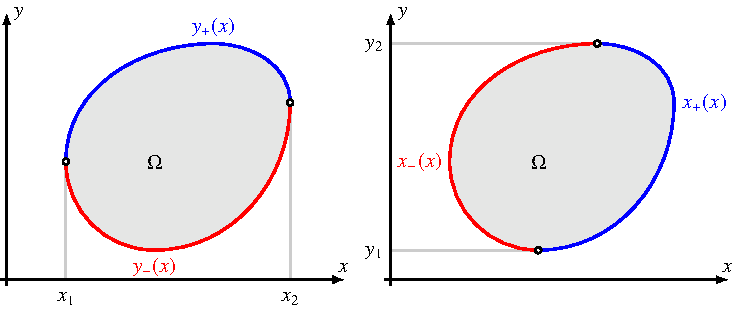
\includegraphics{chapters/040-felder/images/greenbeweis.pdf}
\caption{Beweis des Satzes von Green für ein Gebiet, welches durch
die Graphen zweier Funktionen $y_(x)$ und $y_+(x)$ 
berandet ist.
Alternativ kann das gleiche Gebiet auch durch die Graphen der Funktionen
$x_-(y)$ und $x_+(y)$ berandet werden.
Die Verwendung der beiden Berandungsarten für verschiedene Komponenten
in der Formel von Green ermöglicht den Beweis.
\label{buch:felder:fundamentallemma:fig:greenbeweis}}
\end{figure}

Es genügt damit, den Satz von Green für Gebiete zu beweisen, dessen Rand
aus den Graphen der Funktionen $y_-(x)$ und $y_+(x)$ für den unteren und
oberen Rand und den vertikalen Strecken von $(x_i,y_-(x_i))$ nach
$(x_1,y_+(x_i))$ besteht
(Abbildung~\ref{buch:felder:fundamentallemma:fig:greenbeweis}).

Mit dieser Beschreibung des Gebietes berechnen wir jetzt beide Seiten
von \eqref{buch:felder:fundamentallemma:eqn:green} 
für $g=0$ und zeigen, dass sie gleich sind.
Das Integral des zweiten
Terms des Integranden auf der linken Seite von
\eqref{buch:felder:fundamentallemma:eqn:green} wird zu
\begin{align}
I_l
&=
-\int_{\Omega}
\frac{\partial f}{\partial y}(x,y)
\,dx\,dy
=
-
\int_{x_1}^{x_2}
\int_{y_(x)}^{y_+(x)}
\frac{\partial f}{\partial y}(x,y)
\,dy
\,dx.
\notag
\intertext{Das Integral kann mit dem Hauptsatz der Integralrechung
ausgeführt werden und ergibt}
&=
-
\int_{x_1}^{x_2}
\biggl[ 
f(x,y)
\biggr]_{y_-(x)}^{y_+(x)}
\,dx
=
\int_{x_1}^{x_2}
-f(x,y_+(x))+f(x,y_-(x))
\,dx
\label{buch:felder:fundamentallemma:eqn:greenhaupt}
\end{align}
Die rechte Seite von \eqref{buch:felder:fundamentallemma:eqn:green}
besteht aus vier Teilen, die einzeln berechnet werden können:
\begin{align*}
I_r
&=
\int_{x_1}^{x_2} f(x,y_-(x)),dx
+
\int_{y_-(x_2)}^{y_+(x_2)} \underbrace{g(x,y)}_{\displaystyle=0}\,dy
+
\int_{x_2}^{x_1} f(x,y_+(x))\,dx
+
\int_{y_+(x_1)}^{y_-(x_1)} \underbrace{g(x,y)}_{\displaystyle=0}\,dx
\intertext{Es bleiben nur der erste und dritte Term stehen, die zusammen
das Gleiche ergeben wir $I_l$:}
&=
\int_{x_1}^{x_2} f(x,y_-(x))\,dx
-
\int_{x_1}^{x_2} f(x,y_+(x))\,dx
=
I_l.
\end{align*}
Damit ist die Formel~\eqref{buch:felder:fundamentallemma:eqn:green}
für $g=0$ beweisen.

Um die Formel~\eqref{buch:felder:fundamentallemma:eqn:green} auch
für $f=0$ und $g\ne 0$ zu beweisen, geht man gleich vor mit 
einer Zerlegung des Gebietes in horizontale Streifen.
Da die Formel linear ist in $f$ und $g$ folgt die Behauptung.
\end{proof}

Der entscheidende Schritt im Beweis war die Anwendung des Hauptsatzes
der Integralrechnung in
\eqref{buch:felder:fundamentallemma:eqn:greenhaupt}.
Damit wird auch gerechtfertigt, dass der Satz von Green eine Art
Erweiterung des Hauptsatzes auf zweidimensionale Gebiet ist.

%
% Der Satz von Gauss
%
\subsubsection{Der sSatz von Gauss}
Der Satz~\ref{buch:felder:fundamentallemma:satz:green} von Green
war das erste Beispiel eines Satzes, der ein Gebietsintegral über eine
``abgeleitete Funktion'' in ein Randintegral umzuwandeln gestattet, wobei
die Ableitung wegfällt.
Der Beweis wie auch die Formulierung des Satzes gehen von einer
zweidimensionalen Situation aus und es ist nicht offensichtlich,
wie die Verallgemeinerung auf höhere Dimensionen zu formulieren wäre.
Die Antwort gibt der folgende Satz von Gauss.

\begin{satz}[Gauss]
\label{buch:felder:fundamentallemma:satz:gauss}
\index{Gauss!Satz von}
\index{Satz!von Gauss}
Ist $g(x)$ ein stetig differenzierbares Vektorfeld auf einem Gebiet
$\Omega$ mit glattem Rand $\partial\Omega$ dann gilt
\begin{equation}
\int_\Omega \operatorname{div}g(x)\,dx
=
\int_{\partial\Omega} g(x)\cdot do(x),
\label{buch:felder:fundamentallemma:eqn:gauss}
\end{equation}
wobei das zweite Integral der Fluss des Vektorfeldes $g(x)$ durch
die Randfläche ist.
\end{satz}

\begin{proof}
Der Beweis des Satzes von Stokes war dadurch erfolgreich, dass für jeden
Term des Integranden eine andere, speziell gut geeignete Zerlegung
des Integrationsgebietes gewählt werden konnte, mit der das Integral
mit Hilfe des Hauptsatzes der Integralrechnung vereinfacht werden konnte.
Diese Vorgehensweise führt auch im vorliegenden Fall zum Erfolg.

Wir zerlegen das Integrationsgebiet in zylindrische ``Säulen'', die
oben und unten durch die Graphen der Funktionen $z_-(x,y)$ und $z_+(x,y)$ 
berandet sind.
Der Grundriss der Säule ist ein 2-dimensionales Gebiet $G$.
Der Rand einer solchen Säule besteht dann zusätzlich noch aus der
Mantelfläche, deren Normale aber überall senkrecht auf dem Standarbasisvektor
$\vec{e}_3$ ist.

Wir im Satz von Stokes berechnen wir die linke Seite von
\eqref{buch:felder:fundamentallemma:eqn:gauss} für eine Säule und erhalten
\begin{align*}
I_l
&=
\int_\Omega \operatorname{div}g(x)\,dx
=
\int_{G}\int_{z_-(x,y)}^{z_+(x,y)}
\frac{\partial g_3}{\partial z}(x,y,z)
\,dz\,dx\,dy
\\
&=
\int_G \biggl[ g_3(x,y,z)\biggr]_{z_-(x,y)}^{z_+(x,y)}\,dx\,dy
=
\int_G g_3(x,y,z_+(x,y)) - g_3(x,y,z_-(x,y)) \,dx\,dy
\end{align*}
Die rechte Seite ist ein Oberflächenintegral über die drei früher
identifizierten Teile der Oberfläche, wobei der Teil über die Mantelfläche
verschwindet, weil die Normale auf die Mantelfläche senkrecht auf dem
Vektor $g(x,y,z)$ steht.
Es müssen daher nur die Endflächen berücksichtigt werden.
Das Flächenelement auf der Fläche $z(x,y)$ ist 
\[
\begin{pmatrix}
1\\
0\\
\frac{\partial z}{\partial x}
\end{pmatrix}
\times
\begin{pmatrix}
0\\
1\\
\frac{\partial z}{\partial y}
\end{pmatrix}
\,dx\,dy
=
{\renewcommand{\arraystretch}{1.8}
\begin{pmatrix}
\displaystyle
-\frac{\partial z}{\partial y}\\
\displaystyle
-\frac{\partial z}{\partial x}\\
1
\end{pmatrix}}
\,dx\,dy.
\]
Für die untere Endfläche muss die Normale mit dem entgegegengesetzten 
Vorzeichen gewählt werden, damit sie nach aussen zeigt.
Damit wird das Integral über die Endflächen
\begin{align*}
I_r
&=
\int_{\partial\Omega} g(x) \cdot do(x)
=
\int_{G} g_3(x,y,z_+(x,y)) \,dx\,dy
-
\int_{G} g_3(x,y,z_-(x,y)) \,dx\,dy.
\end{align*}
Dies stimmt mit $I_l$ überein, was den Satz von Gauss für ein
Vektorfeld mit $g_1(x,y)=g_2(x,y)=0$ beschreibt.

Indem man Zylinder mit Achsenrichtungen parallel zu anderen
Koordinatenrichtungen verwendet, kann man den Satz von Gauss auch für
jede andere Komponente des Vektorfeldes $g(x)$ beweisen.
Da die Formel~\eqref{buch:felder:fundamentallemma:eqn:gauss} 
linear in $g(x)$ ist, folgt die allgemeine Formel.
\end{proof}

Der Satz von Gauss gilt noch etwas allgemeiner auch für Integrale der
Divergenz eines $n$-dimensionalen differenzierbaren Vektorfeldes über
ein $n$-dimensionales Gebiet.
Der Beweis bleibt ist mutatis mutandis auch auf die allgemeinere Situation
anwendbar.

Der Satz von Gauss ermöglicht also, einen Divergenz-Operator loszuwerden,
indem man zu einem Integral über den Rand übergeht.

%
% Der Satz von Stokes
%
\subsubsection{Der Satz von Stokes}

\begin{satz}[Stokes]
\label{buch:felder:fundamentallemma:satz:stokes}
\index{Satz!von Stokes}%
\index{Stokes!Satz von}%
Sei $g(x)$ ein stetig differenzierbares, dreidimensionales Vektorfeld
und $S$ eine zweidimensionale Fläche, die von der geschlossenen
Kurve $\partial S$ berandet ist.
Dann gilt
\[
\int_S \operatorname{rot} g(x)\,do(x)
=
\oint_{\partial S} g(x)\cdot ds,
\]
wobei das erste Integral der Fluss des Vektorfeldes $\operatorname{rot}g$
durch die Fläche $S$ und das zweite Integral des Pfadintegral des
Vektorfeldes entlang der Randkurve ist.
\end{satz}

